\documentclass[a4paper, 12pt]{article}
\usepackage[left=1.5cm, text={18cm, 25cm}, top=2.5cm]{geometry}
\usepackage[utf8]{inputenc}
\usepackage[czech]{babel}
\usepackage{cite}
\usepackage{graphicx}
\usepackage{float}
\usepackage{amsmath}
\usepackage{tikz}
\usepackage{url}
\newcommand{\myuv}[1]{\quotedblbase #1\textquotedblleft}
\newcommand{\defVal}[1]{$Default=#1$}

\title{Optimalizační algoritmus ACO}
\author{Martin Hruška\\xhrusk16@stud.fit.vutbr.cz}

\date{}
\begin{document}

\maketitle

\section{Úvod}
\label{sec:intro}
Ant colony optimization (ACO), neboli Optimalizace mravenčí kolonií je optimalizační meta-heuristika řadící se do oboru umělé inteligence,
konkrétně patřící mezi metody inteligence hejna. Algoritmus hledá optimální řešení pomocí vzájemně komunikujících agentů (umělých mravenců), kteří
inkrementálně hledají nejlepší cestu grafem s~oceněnými hranami \cite{aco:main}. 
Z~tohoto důvodu musí být optimalizační problém popsatelný právě oceněným grafem, tudíž se metoda používá především pro řešení diskrétních problémů.

Cílem této práce je vytvoření nástroje pro demonstraci činnosti ACO algoritmu, který umožní s~algoritmem experimentovat, zároveň bude jednoduše rozšiřitelný
o~další modifikace algoritmu, ale již v~základní verzi bude implementovat více verzí algoritmu. Implementačním jazykem je C++ a bude použit objektově orientovaný
přístup pro zvýšení modifikovatelnosti a rozšiřitelnosti kódu. Nástroj bude mít podobu konzolové aplikace.

V~tomto dokumentu bude popsán samotný algoritmus (sekce \ref{sec:algorithm}), dále architektura a implementace samotného programu (sekce \ref{sec:design}),
experimenty provedené s~algoritmem a jejich vyhodnocení (sekce \ref{sec:eval}).
Součástí dokumentu jsou tři přílohy obsahující návod k~instalaci (doplněk \ref{app:install}),
uživatelskou příručku (doplněk \ref{app:help}) a popis formátu vstupního grafu (doplněk \ref{app:format}).

\section{ACO Algoritmus}
\label{sec:algorithm}
Jak bylo uvedeno v~úvodní sekci \ref{sec:intro}, algoritmus pracuje s~množinou mravenců, kteří inkrementálně řeší daný optimalizační problém tak, že
v~jednotlivých iteracích hledají optimální cestu ve váženém grafu popisujícím daný problém. Za řešení úlohy se považuje cesta (posloupnost vrcholů grafu)
procházející všemi vrcholy grafu právě
jednou s~tím, že se mravenec nakonec cesty vrací do počátečního uzlu. Každá hrana grafu má určitou hladinu feromonu, který vypouští mravenci při každém průchodu.
Feromon  ovlivňuje výběr hrany pro další krok mravence při tvorbě řešení v~dané iteraci.
Existují různé varianty ACO algoritmu, nyní bude ovšem popsána jeho základní verze nazvaná Ant System.

Řešení optimalizačního problému probíhá v~zadaném počtu iterací, při čemž v~každé iteraci vytvoří každý mravenec svoje řešení.
Počáteční uzel, ze kterého mravenec začíná vytvářet cestu, je vybrán náhodně.
V~každém kroku tvorby řešení musí mravenec zvolit další hranu, po níž bude pokračovat do dalšího uzlu. Volba hrany záleží na ceně této hrany (tedy vzdálenosti
uzlu, do kterého tato hrana vede) a hladině feromonu na dané hraně. Tyto dvě veličiny určují pravděpodobnost,
se kterou si mravenec vybere danou hranu dle následujícího vzorce \cite{aco:variations}:
\begin{center}
  $p(c_{ij}|s_k^p) =
   \begin{cases} 
      \frac{\tau^{\alpha}_{ij}\eta^{\beta}_{ij}}{\sum\limits_{c_{il}\in N(s_k^p)}{\tau^\alpha_{il}\eta^\beta_{il}}} & j \in N(s_k^p) \\
      0 & otherwise 
   \end{cases}
   $
\end{center}
kde $c_{ij}$ je hrana z~uzlu $i$ do uzlu $j$, $s_k^p$ je částečné řešení mravence $k$, $N(s_k^p)$ je množina vrcholů nepatřících do $s_k^p$, $\eta_{ij}$ je 
dáno vztahem ($1/d_{ij}$), $d_{ij}$ je cena hrany (vzdálenost) mezi uzly $i$ a $j$, $\tau_{ij}$ je hladina feromonu na hraně $c_{ij}$, $\alpha$
je váha feromonu a $\beta$ je váha vzdálenosti mezi $i$ a $j$.

Jakmile jsou řešení pro dané mravence hotova, najde se mravenec s~nejkvalitnějším řešením v~dané iteraci a pokud je toto lepší, než aktuálně nejlepší řešení
z~doposud provedených iterací, tak je uloženo na jeho místo.

Hladina feromonu je aktualizována na konci každé iterace a to tak, že mravenec vypouští po cestě, kterou prošel grafem, množství feromonu přímo úměrné kvalitě
ním vytvořeného řešení. V~různých verzích algoritmu se technika aktualizace feromonu, množství feromonu vypouštěného mravencem, či počet mravenců vypouštějících 
feromon může různit. V~popisované verzi Ant System je feromon na hraně z~vrcholu $i$ a $j$ aktualizován následujícím způsobem \cite{aco:variations}:
\begin{center}
  $\tau_{ij}=(1-\rho)\tau_{ij}+\sum\limits_{k=1}^{n}\Delta\tau_{ij}^k$
\end{center}
kde $\rho \in <0,1>$ je koeficient odpařování feromonu
a $\Delta\tau_{ij}^k$ je množství feromonu přidaného na hranu z~$i$ do $j$ $k$-tým mravencem a je definováno následovně:
\begin{center}
  $\Delta\tau_{ij}^k = 
  \begin{cases}
    \frac{Q}{L_k} & \emph{pokud je hrana } ij \emph{ v~řešení k-tého mravence}\\
    0 & jinak
   \end{cases}
   $
\end{center}
kde $Q$ je konstanta udávající množství feromonu vyloučeného jedním mravence v~jedné iteraci a $L_k$ je cena řešení (t.j. délka cesty) $k$-tého mravence.

Algoritmus je prováděn, dokud není dosažen počet iterací zadaný uživatelem.

\subsection{Modifikace}
\label{subsec:modif}
V~předchozí částí byl popsán ACO algoritmus v~jeho základní verzi -- Ant System. Existují ovšem modifikace tohoto přístupu.
V~následující části dokumentu budou popsány napřed modifikace Ant System algoritmu a to Ant Density, Ant Quantity, Elitist Strategy, dále budou
také uvedeny alternativní ACO algoritmy k~Ant System a to Ant Colony System, Max-Min System a Rank-based System. Veškerá notace v~této části odpovídá
definicím zavedeným v~předchozím textu.

\subsubsection{Ant Density}
Jedná se o~modifikaci Ant system, kde je hodnota $\Delta\tau_{ij}^k$ (množství feromonu přidaného na hranu z~$i$ do $j$ $k$-tým mravencem) definována
následovně \cite{aco:variations}:
\begin{center}
  $\Delta\tau_{ij}^k = 
  \begin{cases}
    Q & \emph{pokud je hrana } ij \emph{ v~řešení k-tého mravence}\\
    0 & jinak
   \end{cases}
   $
\end{center}

\subsubsection{Ant Quantity}
Jde opět o~modifikaci Ant System upravující definici $\Delta\tau_{ij}^k$ (množství feromonu přidaného na hranu z~$i$ do $j$ $k$-tým mravencem) na následující
tvar \cite{aco:variations}:
\begin{center}
  $\Delta\tau_{ij}^k = 
  \begin{cases}
    Q/d_{ij} & \emph{pokud je hrana } ij \emph{ v~řešení k-tého mravence}\\
    0 & jinak
   \end{cases}
   $
\end{center}

\subsubsection{Elitist Strategy}
Elitist Strategy je další z~variací Ant System. Je založena na odlišné aktualizaci feromonové stopy na cestě, která je prozatím vybrána jako nejlepší.
Hrany této cesty jsou aktualizovány dle následujícího vztahu\cite{aco:variations}:
\begin{center}
  $\tau_{ij}=(1-\rho)\tau_{ij}+\sum\limits_{k=1}^{n}\Delta\tau_{ij}^k + e*Q/L^*$
\end{center}
kde $e$ je počet mravenců, kteří prošli přes hranu $ij$ (která patří do nejkratší cesty), $L^{*}$ je délka nejlepší cesta.

Hrany, které nepatří do nejlepší cesty, jsou aktualizovány dle vztahu uvedeného výše v~části \ref{sec:algorithm}.

\subsubsection{Ant Colony System}
Ant Colony System je po Ant System další algoritmus založený na ACO. Přístup k~aktualizaci feromonu na hranách zůstal zachován, ale byl změněn způsob
výběru dalšího vrcholu, do kterého má pokračovat mravenec při tvorbě svého řešení v~dané iteraci. Výběr vrcholu $j$ pro další cestu $k$-tého mravence
je proveden následovně \cite{aco:acs}:
\begin{center}
  $j = 
  \begin{cases}
    \arg\max\limits_{u\in N(s^p_k)}\tau_{iu}\eta^{\beta}_{iu} & if\ q\leq q_0\\
    \emph{Výběr dle pravděpodobnosti stejně jako v~AS} & jinak
   \end{cases}
   $
\end{center}
kde $q_0\in (0,1)$ je předem zadaný parametr a $q$ náhodné číslo generované pomocí uniformního rozložení z~intervalu $<0,1>$.

\subsubsection{Max-Min Ant System}
Max-Min Ant system je dalším ACO algoritmem. Od Ant System se odlišuje způsobem aktualizace feromonu na hranách a to tak, že feromon vypouští pouze
nejlepší mravenec (označme ho \emph{best}). Aktualizace feromonu na hranách je pak prováděna následovně \cite{aco:maxmin}:
\begin{center}
  $\tau_{ij}=(1-\rho)\tau_{ij}+\Delta\tau_{ij}^{best}$
\end{center}
kde $\Delta\tau_{ij}^{best}=\frac{1}{L_{best}}$ a hrana $ij$ je v~nejlepší cestě dané iterace.

Hodnota feromonu je pak upravena tak, že přesahuje-li předem danou maximální hranici, je na ni zmenšena. Symetricky toto platí pro minimální hranici. Formálně
zapsáno \cite{aco:maxmin}:
\begin{center}
  $\tau_{ij} = 
  \begin{cases}
    \tau_{ij} & \tau_{min} < \tau_{ij} < \tau_{max}\\
    \tau_{min} & \tau_{min} \geq \tau_{ij}\\
    \tau_{max} & \tau_{max} \leq \tau_{ij}\\
   \end{cases}
   $
\end{center}
kde $\tau_{min}$ a $\tau_{max}$ jsou předem dané parametry určující minimální, respektive maximální možné hodnoty feromonu na hranách.

\subsubsection{Rank-based Ant System}
Ve variantě Rank-based Ant system provádí aktualizaci feromonu jen předem daný počet nejlepších mravenců, kteří jsou hodnoceny dle délky své cesty.
Navíc je množství feromonu vypouštěného mravencem přímo úměrné kvalitě jeho cesty (t.j. mravenci s~kratší cestou vypouští víc feromonu). Je zřejmé,
že pro účely tohoto algoritmu je nutné mravence seřadit dle délky jejich cesty, kde nejlepší bude nejkratší cesta. Aktualizace feromonu na hranách pak
probíhá takto \cite{aco:ranked}:
\begin{center}
  $\tau_{ij}=(1-\rho)\tau_{ij}+\sum\limits_{k=1}^{\sigma-1}\Delta\tau_{ij}^k + \Delta\tau_{ij}^*$
\end{center}
  kde $\sigma$ je předem zadaný počet nejlepších mravenců, kteří budou vypouštět feromon, a $\Delta\tau_{ij}^k$ je definováno následovně
\begin{center}
  $\Delta\tau_{ij}^k = 
 \begin{cases}
  (\sigma - k)\frac{Q}{L_k} & \emph{pokud je hrana } ij \emph{ v~řešení k-tého mravence}\\
  0 & jinak
 \end{cases}
$
\end{center}
a $\Delta\tau_{ij}^*$ takto:
\begin{center}
$\Delta\tau_{ij}^* = 
 \begin{cases}
  \sigma\frac{Q}{L^*} & \emph{pokud je hrana } ij \emph{ v~nejlepší cestě}\\
  0 & jinak
 \end{cases}
   $
\end{center}
kde $L^*$ je cena nejlepší nalezené cesty.

% jake jsou rozsireni algoritmu
\section{Návrh a implementace}
\label{sec:design}
Aplikace byla ve fázi návrhu rozčleněna do několika logických celků, jenž jsou rozděleny do tříd v~souladu s~metodologií
objektově orientovaného návrhu. Základní logické rozčlenění aplikace, které bude dále popsáno podrobněji, je následující (viz. také obrázek
\ref{img:logika}):
\begin{itemize}
  \item Zpracování parametrů příkazového řádku
  \item Zpracování vstupního souboru s~grafem
  \item Interní reprezentace grafu
  \item Generování a reprezentace mravenců
  \item Implementace ACO algoritmu
\end{itemize}

\begin{figure}[b]
  \begin{center}
    \begin{tikzpicture}[
  node distance = 4cm,
  block_main/.style={rectangle, text centered, rounded corners, thick, fill=blue!50,
    minimum height = 5em, minimum width = 5em},
  block/.style={rectangle, text centered, rounded corners, thick, fill=orange!50,
    minimum height = 5em, minimum width = 5em, text width = 6em},
  line/.style={draw, -}
  ]

\node [block_main] (main) {main()};
\node [block, right of=main] (param) {Zpracování\\parametrů};
\node [block, above of=param, right of=main] (graph_pars) {Zpracování vstupního grafu};
\node [block, left of=graph_pars] (graph) {Interní reprezentace grafu};
\node [block, left of=main] (ants) {Populace mravenců};
\node [block, left of=graph] (aco) {Implementace ACO algoritmu};

\path [line] (main) -- (param);
\path [line] (main) -- (graph_pars);
\path [line] (main) -- (graph);
\path [line] (main) -- (aco);
\path [line] (main) -- (ants);

\path [line] (graph) -- (graph_pars);
\path [line] (graph) -- (aco);
\path [line] (aco) -- (ants);
\path [line] (graph) -- (ants);
\end{tikzpicture}

  \end{center}
\caption{Základní logické rozčlenění aplikace}
\label{img:logika}
\end{figure}


\subsection{Zpracování parametrů příkazového řádku}
\label{subsec:process}
Parametry ACO algoritmu a další volby je možné nastavit prostřednictvím parametrů příkazového řádku. Jejich bližší popis lze nalézt v~doplňku \ref{app:help}.
Pro zpracování těchto parametrů byly navrženy následující dvě třídy:
\begin{itemize}
  \item \emph{Parameters}: Uchovává hodnoty všech parametrů převedené do příslušných datových typů.
  \item \emph{ParametersParser}: Zpracovává zadané parametry a nastavuje dle nich objekt třídy \emph{Parameters}.
\end{itemize}

\subsection{Zpracování vstupního souboru s~grafem}
Pro zpracování vstupního grafu (jeho formát viz. \ref{app:format}) a jeho převedení do interní reprezentace (třída \emph{Graph}) slouží tato třída:
\begin{itemize}
  \item \emph{GraphParser}
\end{itemize}

\subsection{Interní reprezentace grafu}
\label{subsec:graph}
Graf je interně reprezentován pomocí následujících tříd:
\begin{itemize}
  \item \emph{Graph}: Třída uchovává jako datové členy množiny hran (objekty třídy \emph{Edge}) a vrcholů (objekty třídy \emph{Vertex}).
    Umožňuje také zpětnou serializaci grafu do textové podoby metodou \emph{serialize}.

  \item \emph{Vertex}: Třída reprezentující vrchol v~grafu. Obsahuje seznam objektů třídy \emph{Edge} reprezentující hrany, které spojují daný vrchol s~danými
    vrcholy.

  \item \emph{Edge}: Třída reprezentující hranu grafu. V~datových členech mimo jiné uchovává vrcholy, které spojuje,
    a mravence, které přes ni v~dané iteraci prošli. Třída také obsahuje metodu pro aktualizaci hladiny feromonu na hraně
    (popis této operace v~sekci \ref{sec:algorithm}).
\end{itemize}

\subsection{Populace mravenců}
Základem ACO algoritmu je populace mravenců, kteří postupně tvoří optimální řešení daného problému. Pro práci s~populací mravenců byly navrženy tyto dvě třídy:
\begin{itemize}
  \item \emph{Ant}: Třída popisující umělé mravence. Obsahuje metody pro výběr dalšího uzlu během tvorby řešení a také uchovává informace o~řešení
  tvořeném mravencem
    v~aktuální iteraci.
  \item \emph{AntPopulation}: Generuje a uchovává populaci mravenců.
\end{itemize}

\subsection{Implementace ACO algoritmů}
Jak bylo popsáno v~části \ref{sec:algorithm}, existuje více algoritmů implementujících ACO meta-heuristiku.
Aplikace implementuje všechny z~popsaných variant algoritmu a to pomocí těchto tříd 

\begin{itemize}
  \item \emph{ACOAlgorithm}: Zastřešuje provádění ACO algoritmu a jeho hlavních částí, tedy tvorby řešení mravenců v~dané iteraci,
  uložení nejlepšího řešení a také aktualizaci feromonu. Pro konkrétní provedení těchto operací volá metody třídy \emph{ASImplementation} a jejich potomků.
  \item Hlavní třídou implementující konkrétní operace je \emph{ASImplementation}, která implementuje Ant System v~jeho základní podobě. Tuto třídu
  dědí ostatní třídy implementující jiné varianty ACO a případně pomocí polymorfismu upravují ty části algoritmu, v~které se daná varianta liší. Implementovány
  byly ještě následující třídy:
    \begin{itemize}
      \item \emph{ASDensity} -- implementuje verzi Ant System density.
      \item \emph{ASQuantity} -- implementuje verzi Ant System quantity.
      \item \emph{ASElitist} -- implementuje elitářskou variantu Ant System.
      \item \emph{ASAcs} -- implentuje Ant Colony System.
      \item \emph{ASMaxMin} -- implementuje MaxMin Ant System.
      \item \emph{ASRanked} -- implementuje Rank-based Ant System.
    \end{itemize}
\end{itemize}

\subsection{Upřesnění ACO algoritmu}
Během implementace byly učiněny následující zpřesnění ACO algoritmu k~popisu ze sekce \ref{sec:algorithm}.
\begin{itemize}
  \item Pokud během výběru dalšího uzlu při tvorbě řešení jednotlivých mravenců má více vrcholů stejnou pravděpodobnost výběru, tak je jeden z~nich vybrán náhodně.
  Tím se předchází opakovanému procházení stejné cesty jen kvůli specifickému seřazení uzlů v~interní reprezentaci.
  \item Jako vstup je akceptován i neúplný graf, tudíž může během tvorby řešení dospět některý z~mravenců do uzlu, z~něhož již nemá další cestu. Takovýto mravenec
  je po zbytek iterace ignorován a to včetně aktualizace feromonu na hranách.
  \item S~předchozím bodem souvisí také to, že pokud žádný mravenec nenalezne během zadaných iterací korektní řešení, může algoritmus skončit bez nalezení
  řešení.
\end{itemize}

\subsection{Vývojové prostředí a nástroje}
Implementace byla provedena v~jazyce C++ bez použití externích knihoven. Program byl vyvíjen a testován na systému Linux (distribuce Debian Wheezy) a na školním
serveru \emph{merlin.fit.vutbr.cz}.

\section{Experimenty a vyhodnocení}
\label{sec:eval}
% popsat nejaky rozumny graf/nakreslit ho -> udelat graf vzadelnosti odchylek v zavislosti na poradi prochazky
Aplikace byla testována na problému obchodního cestujícího. Grafy, pomocí nichž je problém zadán, byly získány z~TSPLIB \cite{TSPLIB}.
Použité grafy lze najít ve složce \emph{examples/}, kde jsou již grafy konvertovány do vstupního formátu pro dokumentovanou aplikaci. Pro bližší popis
byla vybrána úloha \emph{d198}, se kterou již byly provedeny experimenty v~\cite{aco:maxmintsp,aco:acs}. V~následujících experimentech byly použity tyto
parametry:
  \begin{itemize}
    \item $\alpha=1, \beta=2, \rho=0.2$
    \item Počet mravenců: 25
    \item Počet iterací: 1000
  \end{itemize}
Pokud jsou uváděny průměrné hodnoty, jsou tyto průměry vypočteny z~minimálně 15 měření.
% provedl jsem ho

\subsection{d198}
Tato varianta úlohy obsahuje 198 vrcholů grafu, přes které se hledá optimální cesta. Pro experiment byly použity dvě varianty algoritmu:
\begin{itemize}
  \item MaxMin Ant System, kde jako minimum byla zvolena hodnota $0.000001$ a jako maximum $0.000473$ a to dle vztahu z~\cite{aco:maxmintsp}.
  \item Ant Colony System, kde hodnota $q_0=0.95$ stejně jako v~\cite{aco:acs}.
\end{itemize}
Výsledky experimentů jsou shrnuty v~tabulce \ref{tabd198}. Optimálním řešením tohoto problému je $15 780$ \cite{aco:acs}.
\begin{table}[tb]
\begin{center}
  \begin{tabular}{ | l | r | r |}
   \hline
    & \textbf{Nejlepší výsledek} & \textbf{Průměrný výsledek} \\ \hline \hline
    ACO MaxMin & $16138$ & $16560.5$ \\ \hline
    ACO ACS & $16803$ & $17520.2$ \\ \hline
    ACS z~\cite{aco:acs} & $15 780$ & $15 781.7$ \\ \hline
    MaxMin z~\cite{aco:maxmintsp} & $15 780$ & $15 780.2$\\ \hline
   \end{tabular}
   \caption{Tabulka výsledků experimentu s~úlohou d198.}
   \label{tabd198}
\end{center}
\end{table}
Jak je patrno z~výsledků implementace algoritmu z~\cite{aco:maxmintsp,aco:acs} byly schopny nalézt optimální řešení, dokumentovaná aplikace nikoliv a nejlepší
výsledek $16138$, který nalezla, se lišil
od optimálního řešení se lišila o~$2.26\%$ \footnote{Odchylka vypočítána dle vztahu $\frac{(\emph{výsledek}-\emph{optimum})}{\emph{optimum}}*100$}. To lze
přisoudit použití dalších heuristik jako \emph{zrychlení aktualizace feromonu, kandidátní list, lokálního prohledávání}
v~implementacích z~\cite{aco:maxmintsp,aco:acs}, alespoň dle experimentů provedených s~nástrojem \emph{ACOTSP} \footnote{nástroj je dostupný na
\url{http://iridia.ulb.ac.be/~mdorigo/ACO/aco-code/public-software.html}} bez a s~použitím příslušných optimalizací.

Graf \ref{fig:best} dokumentuje konvergenci k~optimálnímu řešení, které bylo nalezeno algoritmem MaxMin Ant System během jednoho z~pokusů.
Na ose $x$ je pořadí iterace a na ose $y$ cena nejlepšího řešení v~dané iteraci. Je patrné, že přibližně od 500. iterace již mravenci v~další iteracích lepší řešení
nenacházeli, nýbrž vždy dospěli k~(lokálnímu) optimu.

\begin{figure}[bt]
\begin{center}
\scalebox{0.6}
{
  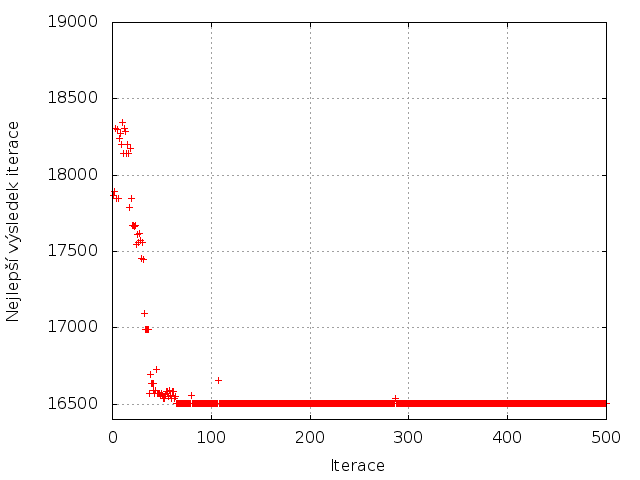
\includegraphics{imgs/best.png}
}
\caption{
Konvergence k~optimálnímu řešení \emph{d198} během jednotlivých iterací.}
\label{fig:best}
\end{center}
\end{figure}

\subsubsection{lin318}
Další experiment byl proveden s~úlohou \emph{lin318}, jež obsahuje $318$ vrcholů. Cena optimálního řešení této úlohy je $42029$ \cite{aco:acs}. Výsledky experimentu
a porovnání s~\cite{aco:maxmintsp,aco:acs} lze najít v~tabulce \ref{tablin318}.
\begin{table}[tb]
\begin{center}
  \begin{tabular}{ | l | r | r |}
   \hline
    & \textbf{Nejlepší výsledek} & \textbf{Průměrný výsledek} \\ \hline \hline
    ACO MaxMin & $16138$ & $16560.5$ \\ \hline
    ACO ACS & $16803$ & $17520.2$ \\ \hline
    ACS z~\cite{aco:acs} & $42 029$ & $42 029$ \\ \hline
    MaxMin z~\cite{aco:maxmintsp} & $42 029$ & $42 029$\\ \hline
   \end{tabular}
   \caption{Tabulka výsledků experimentu s~úlohou lin318.}
   \label{tablin318}
\end{center}
\end{table}
Nejlepší výsledek nalezený programem $16138$ se tedy odlišuje od optima o~$X procent$. Důvody tohoto již byly uvedeny výše.

Na grafu \ref{fig:best_lin} je znázorněna konvergence k~optimálnímu řešení během jednotlivých iterací. Na ose x je uvedeno pořadí iterace a ose y
cena nejlepšího řešení v~dané iteraci. Graf \ref{fig:best_lin} je založen na jednom z~běhů algoritmu MaxMin Ant system, které byly provedeny během experimentu.
Tentokrát bylo nalezeno lokální optimum po 300 iteracích a z~něho se algoritmus v~dalších iteracích nedostal.
\begin{figure}[bt]
\begin{center}
\scalebox{0.6}
{
  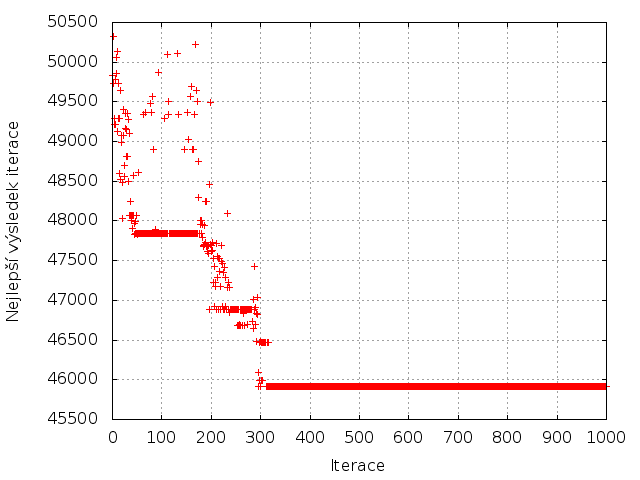
\includegraphics{imgs/best_lin.png}
}
\caption{
Konvergence k~optimálnímu řešení \emph{lin318} během jednotlivých iterací.}
\label{fig:best_lin}
\end{center}
\end{figure}

\subsubsection{rat783}
Posledním popsaným experimentem je řešení úlohy \emph{rat783}. Jako jediný z~úloh použitých pro experimentování není přiložena ve složce \emph{examples/}
kvůli její přílišné velikosti.
Ta obsahuje $783$ vrcholů a cena jejího optimálního řešení je $8 806$ \cite{aco:acs}. 
Měření a porovnání s~experimenty z~\cite{aco:maxmintsp,aco:acs} je v~tabulce \ref{rat783}
\begin{table}[tb]
\begin{center}
  \begin{tabular}{ | l | r | r |}
   \hline
    & \textbf{Nejlepší výsledek} & \textbf{Průměrný výsledek} \\ \hline \hline
    ACO MaxMin & $16138$ & $16560.5$ \\ \hline
    ACO ACS & $7.5$ & $92.5$ \\ \hline
    ACS z~\cite{aco:acs} & $42 029$ & $42 029$ \\ \hline
    MaxMin z~\cite{aco:maxmintsp} & $42 029$ & $42 029$\\ \hline
   \end{tabular}
   \caption{Tabulka výsledků experimentu s~úlohou rat318.}
   \label{rat783}
\end{center}
\end{table}

Graf \ref{rat783} ilustruje opět konvergenci k~optimálnímu řešení během jednotlivých iterací. Na ose x je uvedeno pořadí iterace a ose y cena nejlepšího
řešení v~dané iteraci. Jedná se o~jeden z~běhů algoritmu Ant System MaxMin provedených během experimentů. Jak je zřejmé, tak po X iteracích se algoritmus
dostal do lokálního optima a lepší řešení nalezeno již nebylo.
\begin{figure}[bt]
\begin{center}
\scalebox{0.6}
{
  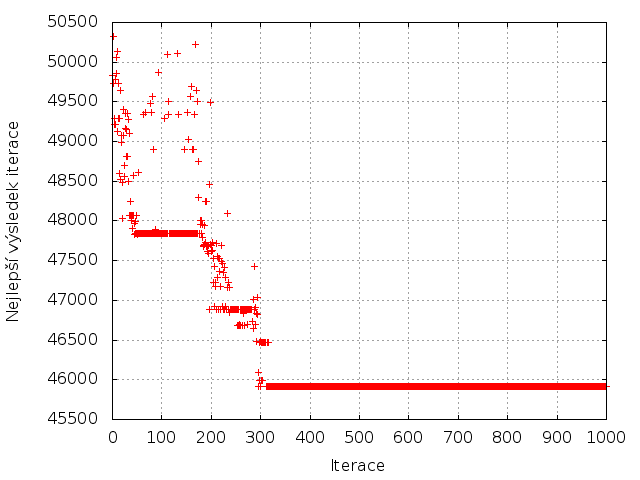
\includegraphics{imgs/best_lin.png}
}
\caption{
Konvergence k~optimálnímu řešení \emph{rat783} během jednotlivých iterací.}
\label{fig:best_rat}
\end{center}
\end{figure}

\section{Závěr}
\label{sec:concl}
Byla implementována konzolová aplikace demonstrující činnost optimalizační meta-heuristiky Ant Colony Optimization. 
Implementována byla základní varianta Ant System, některé
modifikace Ant System, dále také varianta Ant Colony System, MaxMin Ant System a Rank-based Ant System.
Implementace byla provedena v~C++ s~použitím objektově orientovaného přístupu tak, aby by bylo snadné další rozšíření programu o~další varianty ACO.

Aplikace byla testována na několika grafech popisujících problém obchodního cestujícího, v~nichž se ji nepodařilo najít zcela optimální cestu, ale odchylka 
od optima byla v~řádu jednotek procent. Dalším možné rozšíření aplikace spočívá v~implementaci optimalizací
pro získání lepších řešení.

% zhodnit co bylo udelano - knihovna pro experimentovani, snadno rozsiritelna
\newpage
\appendix
\section{Instalace}
K~projektu je přiložen soubor \emph{Makefile}, tudíž lze zdrojové kódy zkompilovat pomocí příkazu \texttt{make}. Pro úspěšnou kompilaci je nutné mít
nainstalovaný překladač GCC. Výstupem kompilace je spustitelný binární soubor \texttt{aco}.
\label{app:install}
\section{Uživatelský manuál}
\label{app:help}
Program lze konfigurovat pomocí parametrů příkazového řádku následujícím způsobem ($Default$ v~popisu parametru udává základní hodnotu,
která bude použita pokud parametr není uživatelem zadán):
\\
\\
  aco -i soubor [parametry]
  \begin{itemize}
  \item Povinné parametry
    \begin{itemize}
      \item -i file ... Cesta k~vstupnímu souboru s~grafem
    \end{itemize}
  \end{itemize}
  \begin{itemize}
    \item Nepovinné parametry parametry
    \begin{itemize}
      \item -v ... Zapne výpisy o~činnosti algoritmu v~každé iteraci algoritmu
      \item -a celé číslo ... Hodnota je počet mravenců v~populaci. \defVal{10}
      \item -m celé číslo ... Počet iterací, které algoritmus provede. \defVal{100}
      \item -p reálné číslo ...  Koeficient $\alpha$. \defVal{1.0}
      \item -d reálné číslo ... Koeficient $\beta$. \defVal{1.0}
      \item -c reálné číslo ... Konstanta $Q$. \defVal{1.0}
      \item -e reálné číslo ... Koeficient $\rho$ z~intervalu $<0,1>$. \defVal{0.5}
      \item -r ... Vypne náhodný výběr z~více vrcholů se stejnou pravděpodobností
      \item -g řetězec ... Použitý ACO algoritmus. Parametr může mít následující hodnoty:
      \begin{itemize}
       \item default ... Základní verze Ant System. Použit jako základní hodnota parametru
       \item density ... Ant System Density
       \item quantity ... Ant System Quantity
       \item elitist ... Ant System Elitist
       \item acs .. Ant Colony System
       \item maxmin ... Max-Min Ant System
       \item ranked ... Rank-based Ant System
      \end{itemize}
      \item Následující parametry jsou závislé na zvoleném algoritmu. Pokud budou použity v~kombinaci s~jiným algoritmem, budou ignorovány.
      \begin{itemize}
        \item -x reálné číslo ... Maximální hodnota feromonu na hraně (Max-Min Ant System). \defVal{0.8}
        \item -n reálné číslo ... Minimální hodnota feromonu na hraně (Max-Min Ant System). \defVal{0.1}
        \item -w reálné číslo ... Počet nejlepších mravenců, kteří vypouští feromon (Rank-based Ant System). \defVal{10}
        \item -q reálné číslo ... Konstanta $q_0$ z~intervalu $<0,1>$ (Ant Colony System).\\\defVal{0.5}
      \end{itemize}
    \end{itemize}
  \end{itemize}
Použité označení u~konstant a koeficientů odpovídá definici v~sekci \ref{sec:algorithm}.

Pro demonstraci běhu programu, nejen získání nejlepšího řešení, se silně doporučuje použití přepínač \emph{-v}.

\subsection{Vstup}
Program čeká jako vstup textový soubor s~popisem grafu, v~němž se bude hledat optimální cesta. Graf musí být popsán ve formátu definovaném 
v~doplňku \ref{app:format}. Ve složce \emph{examples/} jsou příklady grafů, na kterých lze program testovat.

\subsection{Příklad spuštění}
Následující příklad spuštění lze spustit pomocí příkazu \texttt{make run\_example} z~hlavní složky programu:\\
\texttt{./aco -i examples/ex16/ex16.aco -a 10 -m 10 -d 2 -e 0.2 -p 1\\ -g maxmin -x 0.5 -n 0.1 -v}

\section{Formát vstupního souboru}
\label{app:format}
Vstupní soubor bude obsahovat textový popis grafu takový, že na každém řádku bude definována jedna hrana grafu v~následujícím formátu:
\begin{center}
  \texttt{$X$ $Y$ $distance$}
\end{center}
kde $X$, $Y$ jsou vrcholy grafu a $distance$ je vzdálenost mezi nimi. Samotné vrcholy tedy není nutné explicitně definovat. Pokud bude některá hrana
definována vícekrát, je jako rozhodující brána první definice a ostatní jsou ignorovány. Program vypíše v~takovémto případu varování.

\newpage
\bibliography{literatura}
\bibliographystyle{czechiso}
\end{document}
